\documentclass[14pt, a4paper]{report}

%Packages
\usepackage{ngerman}
% TODO make it working\usepackage[german]{babel}
\usepackage{listings}
\usepackage{color}
\usepackage{amssymb}

\usepackage{graphicx}
\usepackage{fancyhdr}
\usepackage{titlesec}
\usepackage{geometry}
%Style
\setlength{\parindent}{0em}

\definecolor{dkgreen}{rgb}{0,0.6,0}
\definecolor{gray}{rgb}{0.5,0.5,0.5}
\definecolor{mauve}{rgb}{0.58,0,0.82}
\definecolor{titleblue}{rgb}{0.21, 0.31, 0.88}

\interfootnotelinepenalty 9999

\lstset{frame=tb,
  language=C++,
  aboveskip=3mm,
  belowskip=3mm,
  showstringspaces=false,
  columns=flexible,
  basicstyle={\small\ttfamily},
  numbers=none,
  numberstyle=\tiny\color{gray},
  keywordstyle=\color{blue},
  commentstyle=\color{dkgreen},
  stringstyle=\color{mauve},
  breakatwhitespace=true,
  tabsize=3
}

\linespread{1.3}

\pagestyle{fancy}
\chead{}
\lhead{\leftmark }
\rhead{}
\cfoot{\thepage}
\lfoot{}
\rfoot{}

\titleformat
{\part} % command
[display]% shape
{\bfseries\huge\center} % format
{Teil  \ \thepart} % label
{0.5ex} % sep 
{\Huge\color{titleblue}} % before-code

\titleformat
{\chapter} % command
[display]% shape
{\color{titleblue}\bfseries\huge\raggedleft} % format
{Kapitel  \ \thechapter} % label
{0.5ex} % sep
{\Huge} % before-code

\titleformat
{\section} % command
[hang]% shape
{\color{titleblue}\bfseries\Large} % format
{}%{Kapitel  \ \thechapter} % label
{0.5ex} % sep
{} % before-code

\newgeometry{left=2.5cm, right=2.5cm }

%Content
\begin{document}

\pagenumbering{roman}

\title{\bfseries \Large Besondere Lernleistung: \\ \Huge \color{titleblue}Simulation eines Zyklotrone am Computer}
\author{Philipp Rosendahl \\ philipp.rosendahl@gmx.de \\ Mallinckrodt-Gymnasium Dortmund}
\date{\today}

\maketitle

\tableofcontents

\chapter{Vorwort}
\pagenumbering{arabic}
\section{Warum simuliert man ein Zyklotron?}
Teilchenbeschleuniger erm"oglichen es Forschern, einen tiefen Einblick in die
Phyisk zu erhalten. Man besch"aftigt sich mit Teilchenbeschleunigern, da sie die
experimentelle Grundlage der Teilchenphysik darstellen. Aber sie sind sehr
teuer und als Sch"uler oder Laie ist es nur schwierig m"oglich, einen
Teilchenbeschleuniger zu benutzen.

Man simuliert Zyklotrone, da man Fehler vorhersagen kann, ohne die Ressourcen
f"ur einen Testlauf aufbringen zu m"ussen. Als Nichtforscher kann man, dank 
Simulationen, einen Einblick in Teilgebiete aktueller Forschung erhalten und risikofrei,
zum Beispiel ohne Zyklotronetrahlung, experimentieren.

\section{Motivation}
Ich m"ochte diese besondere Lernleistung erbringen, da ich es interessant finde, 
zu abstrahieren, Modelle zu entwickeln und diese am PC umzusetzen. 
Teilchenbeschleuniger sind relativ komplex und genie"sen ein gro"ses Interesse
in der "Offentlichkeit, was sie f"ur eine Simulation attraktiv macht. Au"serdem
k"onnte die Simulation im Rahmen des Physikunterrichtes eingesetzt werden, da dort 
ein preiswertes und risikofreies Experimentieren erw"unscht ist.
\section{Ziel dieser Arbeit}
Das Ergebnis dieser Arbeit soll ein Programm sein, mit dem man klassische und 
relativistische Mechanik simuliert. Dabei geht es um die Beschleunigung des Teilchens.
Zerfallseffekte werden aus Vereinfachungsgr"unden vernachl"assigt, da diese den
Umfang der Arbeit sprengen w"urde.

\part{Physikalische Grundlagen}
\chapter{Das Zyklotron}
\section{Aufbau von Teilchenbeschleunigern}
Man differenziert zwischen drei Arten von Teilchenbeschleunigern \footnotemark
\footnotetext{vergleiche Metzler Physik Seite 234}
\begin{enumerate}
\item
Der \textbf{Linearbeschleuniger} besteht aus Beschleunigungskondensatoren, die linear
oder geradlinig hintereinander angeordnet sind und Teilchen auf 
eine h"ohere Geschwindigkeit bringen. Mit Linearbeschleunigern ist ein hoher
Konfigurationsaufwand verbunden, da viele Einstellungen, z.B der Abstand zwischen allen
Kondensatorplatten und die Frequenz an den Kondensatorplatten eingestellt werden m"ussen.
\item \label{ZyklotronBeschreibungAufbau}
Das \textbf{Zyklotron} besteht aus 2 Halbkreisen (Duanten) zwischen denen ein Kondensator 
angeordnet ist. Es werden 2 Arten von Feldern benutzt. Eimal die magnetischen, mit 
denen die 
Teilchen mit Hilfe der Lorenzkraft auf einer Kreisbahen
gehalten werden, und die elektrischen, 
mit denen die Teilchen w"ahrend des "Ubergangs zwischen den Halbkreisen in dem 
Kondensator beschleunigt werden. Ein Zyklotron hat einen geringen 
Konfigurationsaufwand, da f"ur eine optimale Funktionsweise nur die Frequenz an dem 
Kondesator und die St"arke des Magnetfeldes angepasst werden m"ussen. Diese h"angen nur von der 
Masse und der Ladung des Teilchens ab, die nach der klassischen Vorstellung konstant
sind. Haben die Teilchen einen gewissen Umlaufradius erreicht, werden sie mittels eines 
Kondesators aus dem Zyklotron gelenkt.
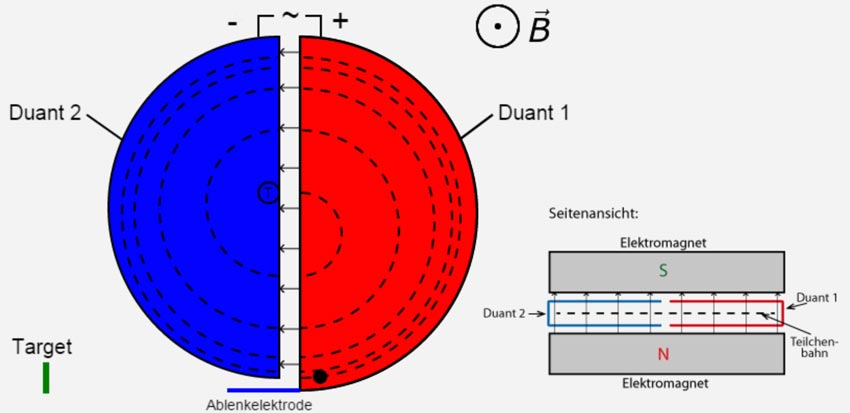
\includegraphics[height=90px]{doc/Aufbau-Zyklotron-de.jpg}
\footnote{http://www.didaktik.physik.uni-muenchen.de/elektronenbahnen/bilder/b-feld/Aufbau-Zyklotron-de.jpg Zugriff: 19.3.2017}

\item
Der \textbf{Synchrotron} ist im Prinzip wie ein Zyklotron aufgebaut mit dem 
Unterschied, dass das Magnetfeld anpassbar ist und in kreisf"ormig angeordneten Rohren 
beschleunigt. Experimente haben gezeigt, dass die
Masse nach Einsteins Relativit"atstheorie keine konstante Gr"o"se ist. Daher muss 
w"ahrend der Beschleunigung das Magnetfeld und die Frequenz an den 
Beschleunigunskondensatoren angepasst werden. Dadurch bleibt eine gute Konfiguration, 
trotz der volatiler Gr"o"sen, erhalten. \label{synchrotron}
\end{enumerate}

\section{Das Zyklotron im Vergleich zu anderen Beschleunigern}
Zyklotrone haben gegen"uber anderen Beschleunigern einige Vorteile: Sie sind einfach
einzustellen, sehr  platzsparend und erm"oglichen durch ihre Kreisform  ein langes
Beschleunigen mit hohen Geschwindigkeiten. Nachteilig ist, dass es eine maximale
Geschwindigkeit gibt und zwingend ein Vorbeschleuniger ben"otigt wird, da sonst das 
Halten der geladenen Teilchen auf der Kreisbahn nicht m"oglich ist. \marginpar{Siehe Lorenzkraft
Seite \pageref {B-Feld-Gleichungen} }

\chapter{Funktion eines Zyklotrone}
\section{Das elektrische Feld}
Das elektrische Feld ist ein mathematisches Modell, mit dem man die Kr"afte zwischen
Ladungen modelliert. Die Feldlinien verdeutlichen dabei die Bewegung von positiver 
Ladung im elektrischen Feld.\footnote{vergleiche Metzler Physik Seite 182}
Dabei verdeutlicht der Abstand zweier
Feldlinien die St"arke des Feldes. F"ur ein Zyklotron betrachten wir nur an"ahernd
homogene elektische Felder, wie sie in einem Kondensator vorkommen. Das Besondere an 
einem homogenen Feld ist, dass die Feldst"arke an jedem Punkt des Feldes gleich stark 
ist. Bei einem Zyklotron stehen die Feldlinien orthogonal auf den Kondensatorplatten
des Beschleunigungskondensators, da dessen Platten parallel zueinander stehen und Ladung
auf ihnen gleichm"a"sig verteilt ist.
F"ur das Feld im Kondensator und auch im Beschleunigungskondesator eines Zyklotrons
sind folgende Beziehungen f"ur diese Simulation wichtig:
\footnote{vergleiche Das Gro"se Tafelwerk interaktiv Seite 107}
\begin{eqnarray} \label{E-Feld-Gleichungen}
\vec{E} = \frac{\vec{F}}{Q} \\
E = \frac{U}{d}
\end{eqnarray}

\section{Das magnetische Feld}
Das magnetische Feld ist, wie das elektrische Feld, auch ein mathematisches Modell.
Allerdings beschreibt dieses nur Wechselwirkungen zwischen bewegten Ladungen. Jede
bewegte Ladung erzeugt ein magnetisches Feld und ein sich "anderndes Magnetfeld 
setzt Ladung in Bewegung. \footnote{elektromagnetische Induktion}
Ein Magnetfeld wirkt auch auf bewegete Ladung. Diese Lorenzkraft l"asst sich als
Rechtssystem definieren:
\newpage
\begin{equation} \label{B-Feld-Gleichungen}
 \vec{F_L} = Q\vec{v} \times \vec{B} \footnotemark
\end{equation}
\footnotetext{vergleiche Metzlers Physik Seite 229}
\begin{equation}
 F_L  = Q * v * B (wenn ~ \vec{v} \perp \vec{B}) \footnotemark
\end{equation}
\footnotetext{vergleiche Das Gro"se Tafelwerk interaktiv Seite 109}

 
\section{Mit elektrischen und magentischen Feldern geladene Teilchen beschleunigen}
In einem Zyklotron werden geladene Teilchen mithilfe elektrischer und magnetischer 
Felder beschleunigt. Dieses ist nur m"oglich, da die Teilchen mit einer
Startgeschwindigkeit $v_0$, die von einem Vorbeschleuniger (meist 
Linerarbeschleuniger) erzeugt wird, in das Zyklotron eintreten. Wie in Kapitel zwei
gezeigt wird 
\marginpar{siehe S. \pageref{ZyklotronBeschreibungAufbau}},
sind f"ur ein Zyklotron 2 Beschleunigungsarten wichtig: erstens eine lineare und 
zweitens eine radiale. F"ur die lineare Beschleunigung, also f"ur die Erh"ohung des 
Betrages der Geschwindigkeit, benutzt man ein elektrisches Feld. Die Feldlinien im 
Kondensator sind an"ahernd parallel zu der Bewegungsrichtung des geladenen Teilchens. 
Also kann angenommen werden, dass die gesamte Kraft auf den Betrag der Geschwindigkeit 
des geladenen Teilchens wirkt. Das magnetische Feld wird dazu verwendet, das geladene
Teilchen auf einer Kreisbahn zu bewegen. Da die Lorenzkraft ein Rechtssystem aus der
Geschwindigkeit, dem Magnetfeld und der Kraft bildet, kann man das Magnetfeld so
in das Zyklotron legen, dass die Lorenzkraft als Zentripitalkraft $F_L = F_Z$ wirkt.
Um das zu erreichen, steht das Magnetfeld immer im rechten Winkel auf der Kreisbahn
des geladenen Teilchens.

Nach der klassischen Vorstellung ist ist die Umlaufzeit eines geladenen Teilchens 
unabh"angig von dessen Geschwindigkeit:
\begin{eqnarray}
  F_L  		&& = F_Z  \footnotemark  \\
  Q * v * B 	&& = \frac{m * v^2}{r} \label{Radius im Zyklotron}\\
  r		&& = \frac{m * v}{Q * B}  ~ | ~ v = \frac{2\pi r}{T} \\
  r		&& = \frac{m * 2 * \pi * r}{Q * B * T} \\
  T		&& = \frac{m * 2 * \pi }{Q * B} \label{klassische_Umlaufzeit}
\end{eqnarray}
\footnotetext{vergleiche Das Gro"se Tafelwerk interaktiv Seite 93}
Alle Werte, von denen die Umlaufzeit $T$ abh"angt, 
sind nach der klassischen Vorstellung konstant. 
Die Frequenz am Beschleunigungskondensator l"asst sich auf genau $f = \frac{1}{T}$
einstellen. Das f"uhrt dazu, dass immer wenn das geladene Teilchen an dem Kondensator 
ankommt, es von dem elektrischen Feld beschleunigt wird. So kann man nach dem klassischen Modell
ein geladenes Teilchen im Prinzip unbegrenzt hoch beschleunigen, bis es aus dem
Zyklotron entfernt wird. \label{klassische_Erwartung}

\chapter{Relativistische Mechanik im Zyklotron}
\section{Grundlage: Relativit"atstheorie}
Neben der klassischen Vorstellung exsistiert allerdings noch die 
Relativit"atstheorie. Einige Ph"anome, wie zum Beispiel die Ergebnissse 
des Michelson-Experimentes,
lassen sich mit der klassischen Vorstellung nicht erkl"aren. Einstein nahm an, dass 
die Gesetze der Elektrodynamik, also auch f"ur elektro-magnetische Wellen wie Licht,
in jedem Inertialsystem gleicherma"sen gelten m"ussen. 
Wenn man sich allerdings mit Lichtgeschwindigkeit bewegt, was in der klassischen Vorstellung 
m"oglich ist, erscheint ein Lichtstrahl als ruhend. 
Die Lichtgeschwindigkeit ist eine Naturkonstante und kann unter keinen 
Umst"anden abweichen. Deshalb postulierte Einstein, dass in jedem Inertialsystem, also in
einem f"ur den Betrachter ruhenden Bezugssystem, die 
Naturkonstanten, wie die Lichtgeschwindigkeit, gleich seien m"ussten. Daraus folgt auch,
dass alle Inertialsysteme bei Beobachtungen und dem Aufstellen von Regeln gleichberechtigt sind. 
Das hei"st, dass man in einem Raumschiff, das mit an"ahernd Lichtgeschwindigkeit
fliegt, die selben Beobachtungen macht, wie auf der Erde.
\footnote{vergleiche Metzler Physik Seite 345}

Daraus folgt, dass einige Gr"o"sen, die nach unserer allt"aglichen Erfahrung konstant
sein m"ussten, nicht konstant sein k"onnen. Nimmt man an, dass man ein Teilchen 
unendlich lange beschleunigt, erreicht man irgendwann den Zeitpunkt, an dem man es nicht weiter
beschleunigen kann, da das Teilchen sonst f"ur einen Moment so schnell wie das Licht 
w"are. Bei weiterem Beschleunigen wird dem Teilchen weiterhin Energie hinzugef"ugt, die 
umgewandelt werden muss. In der klassischen Vorstellung 
w"urde sich die Geschwindigkeit erh"ohen, doch das ist jetzt nicht mehr m"oglich. 
Trotzdem muss die Energie irgendwo gespeichert werden\footnote{Energieerhaltungssatz}. 
Aus der speziellen Relativit"atstheorie leitete Einstein ab, dass die Masse des besagten
Teilchens gr"o"ser wird. In dieser hinzugewonnen Masse wird die Energie gespeichert.
 \marginpar{Variable Masse: Siehe Seite \pageref{var_m} \ref{var_m}}
Dieses Ph"anomen wird erst bei sehr hohen Geschwindigkeiten wahrnehmbar. Die klassische 
Vorstellung trifft auf kleine Geschwindikeiten immer noch n"aherungsweise zu.

So l"asst sich sagen: Aus dem Bezugssystem $S$ betrachtet hat 
ein Objekt im Bezugssystem $S'$ andere Eigenschaften, zum Beispiel eine ver"anderte 
Masse $m_v$, da sich von $S$ aus $S'$ mit einer Geschwindigkeit $v$ bewegt. 
Allerdings funktioniert das auch umgekehrt. Steht der Betrachter im Bezugssystem $S'$,
hat dasselbe Objekt die Ruhemasse $m_0$, w"ahrend sich ein anderes Objekt im System $S$ 
in den Eigenschaften ver"andert hat. Zusammengefasst: Einige Werte, die in der 
klassischen Vorstellung konstant sind, h"angen eigentlich von der Geschwindigkeit 
relativ zum eigenen Bezugssystem ab.

Einige von Einstein abgeleitete Beziehungen sind 
\footnote{vergleiche das Gro"se Tafelwerk interaktiv Seite 116 }:
\begin{eqnarray}
\beta && = \frac{v}{c} \\
\Delta t' && = \Delta t * \sqrt{1 - \beta^2} ~ (Zeitdilatation) \\
\Delta x && = \Delta x' * \sqrt{1 - \beta^2} ~ (L"angenkontraktion) \\
m && = \frac{m_0}{\sqrt{1 - \beta^2}} \label{var_m} \\
W_{ges} && = m * c^2 \label{mc_square}
\end{eqnarray}

\section{Experimenteller Befund: Das klassische Modell schl"agt fehl}
Entgegen den Erwartungen des klassischen Modells
\marginpar{Siehe Seite \pageref{klassische_Erwartung} \ref{klassische_Erwartung}}
lassen sich die Teilchen nicht unbegrenzt beschleunigen. Im klassischen Modell
gilt die Beziehung $T = \frac{m * 2 * \pi }{Q * B}$.
Man ging davon aus, dass sich $T$ nicht ver"andert, da alle Gr"o"sen rechts von dem 
Gleichheitszeichen Konstanten sind. Da sich die Frequenz an dem Kondensator auf
$\frac{1}{T}$ einstellen l"asst, passiert das geladene Teilchen immer dann den Kondensator,
wenn es von dem elektrischen Feld beschleunigt wird. Doch die Masse eines Teilchens
ist keine konstante Gr"o"se \marginpar{vergleiche \ref{var_m}} und steigt mit zunehmender 
Geschwindigkeit. Die Frequenz am Beschleunigungskondensator und die Umlaufzeit $T$ 
wurden
exakt aufeinander abgestimmt, um eine maximale Beschleunigung zu erzielen.
Nun kommt es vor, dass die Spannung im Kondensator sich "andert, w"ahrend sich das 
geladene Teilchen noch in ihm befindet. Das Teilchen wird zun"achst beschleunigt und
dann wieder abgebremst. Man sagt, dass das Zyklotron aus dem Takt ger"at.
Im Extremfall wird der Kondesator genau dann umgepolt, wenn sich das 
Teilchen gerade in der Mitte des Beschleunigungskondensators befindet. Dann wird die 
Geschwindigkeit gar nicht erh"oht, da es genau so lange postiv wie negativ beschleunigt 
wird \footnote{Bremsen wird als negative Beschleunigung betrachtet}.
Aufgrund dieses Befundes wurde das Synchrotron entwickelt.
\marginpar{vergleiche Synchrotron Seite \pageref{synchrotron}}

\chapter{Verwendetes Modell}
\section{Betrachtung der Teilchen, Felder und Bezugssysteme}
\begin{itemize}
\item Teilchen werden in dieser Simulation als Punkte betrachtet, die Masse und Ladung aber keine 
Ausdehung besitzen.
\item Die Felder werden als absolut homogen und perfekt auf die Teilchen ausgerichtet
betrachtet. Man hat also keine Kraftverluste, weil das B-Feld nicht perfekt
orthogonal auf der Kreisbahn der geladenen Teilchen steht.
\item Das Zyklotron wird als Inertialsystem betrachtet.
\end{itemize}

\section{Beschleunigung im E-Feld}
In dieser Simulation wird eine Beziehung der Form $s(t)$ gesucht, mit der man den
Zeitpunkt, an dem das Teilchen den Kondensator verl"asst, mit der Umpolung des 
Kondensators vergleichen kann. Der Ansatz $W_{kin}  = Q * U $ ist daf"ur nicht
hilfreich, da er zeitunabh"angig ist.

Daher verfolgen wir die Interpretation der Kraft als Ableitung des Impulses
\begin{equation}
\dot{p} = f 
\end{equation}
und formen jenen nach einer Gleichung der Gestalt $v(t)$ um, die man zu $s(t)$
integrieren und eine Umkehrfunktion $t(s)$ bilden kann.
\newpage
Es l"asst sich folgender Zusammenhang ableiten:
\begin{eqnarray}
\frac{d}{dt} (m * v ) && = \frac{U * Q}{d} ~~~~~~~~\footnotemark \\
\frac{d}{dt} \left(\frac{m_0 * v}{\sqrt{1 - (\frac{v}{c}})^2}\right) && = \frac{U * Q}{d} \\
\frac{d}{dt} \left(\frac{v}{\sqrt{1 - (\frac{v}{c})^2}}\right) && = \frac{U * Q}{d * m_0} \\
\int_{t_0}^t \frac{d}{dt} \left(\frac{v}{\sqrt{1 - (\frac{v}{c})^2}}\right) 
    && = \int_{t_0}^t \frac{U * Q}{d * m_0} \\
\end{eqnarray}
\begin{center}
$ \frac{U * Q}{d * m_0} $ wird als $ a $ interpretiert \label{Beschleunigung}
\end{center}
\begin{eqnarray}
\frac{v}{\sqrt{1 - \left(\frac{v}{c}\right)^2}} && = a * t + v_0 \\
\frac{v^2}{1 - \left(\frac{v}{c}\right)^2} && = \left(a * t + v_0 \right)^2 \\
v^2  && = \left(a * t + v_0\right)^2 - \left(\frac{v}{c}\right)^2 * \left(a * t + v_0 \right)^2\\
v^2 + \left(\frac{v}{c}\right)^2 * \left(a * t + v_0\right)^2 && = \left(a * t + v_0 \right)^2 \\
v^2 * \left(1 + \frac{(a * t + v_0)^2}{c^2}\right) &&  = \left(a * t + v_0\right)^2 \\
v^2 && = \frac{\left(a * t + v_0\right)^2}{1 + \left(\frac{a * t + v_0}{c}\right)^2} \\ 
v && = \frac{a * t + v_0}{\sqrt{1 + \left(\frac{a * t + v_0}{c}\right)^2}}
\end{eqnarray}
\footnotetext{vergleiche Unkelbachsche Formelsammlung Seite 5 und Seite 15}

\newpage
Nun wird noch ein Zusammenhang f"ur die zur"uckgelegte Streckte im Kondensator formuliert,
um zu berechnen, wie viel Zeit das geladenen Teilchen braucht, um den Kondensator zu
passieren.
\begin{eqnarray}
s(t) && = \int_0^t v(t) ~dt \\
s(t) && = \int_0^t \frac{a * t + v_0}{\sqrt{1 + \left(\frac{a * t + v_0}{c}\right)^2}} ~ dt
\end{eqnarray}

man substuiert $u = 1 + \left(\frac{a * t + v_0}{c}\right)^2$ und 
$dt = \frac{du}{\left(1 + \left(\frac{a * t + v_0}{c}\right)^2\right)\dot{}}$

\begin{eqnarray}
s(t) && = \int_{1 + \left(\frac{v_0}{c}\right)^2}^{1 + \left(\frac{a*t + v_0}{c}\right)^2}  \frac{a * t + v_0}{\sqrt{u}} ~ \frac{du}{ \left({1 + \left(\frac{a * t + v_0}{c}\right)^2}\right)\dot{}}\\
s(t) && =  \int_{1 + \left(\frac{v_0}{c}\right)^2}^{1 + \left(\frac{a*t + v_0}{c}\right)^2}  \frac{a * t + v_0}{\sqrt{u}} ~ \frac{du}{2*\left(\frac{a * t + v_0}{c}\right)*\frac{a}{c}}\\
s(t) && = \frac{1}{2}*\left(\frac{c^2}{a}\right) ~ \int_{1 + \left(\frac{v_0}{c}\right)^2}^{1 + \left(\frac{a*t + v_0}{c}\right)^2} \frac{1}{\sqrt{u}} ~ du \\
s(t) && = \frac{1}{2}*\left(\frac{c^2}{a}\right)~\left[2*\sqrt{u}\right]_{1 + \left(\frac{v_0}{c}\right)^2}^{1 + \left(\frac{a*t + v_0}{c}\right)^2} \\
s(t) && = \left(\frac{c^2}{a}\right) * \left(\sqrt{1 + \left(\frac{a*t + v_0}{c}\right)^2} - \sqrt{1 + \left(\frac{v_0}{c}\right)^2}\right)
\end{eqnarray}

Um die Zeit im Kondensator zu berechnen wird eine Funktion der Gestalt $t_{v_0}(s)$
gesucht, die sich aus der obigen Gleichung $s(t)$ ableiten l"asst. Da die Injektivit"at 
\footnotemark \footnotetext{vergleiche http://www.mathepedia.de/Injektion.aspx letzter Zugriff 19.3.2017} von $s(t)$ nicht gegeben ist, wird eine 
Umkehrfunktion f"ur den Wertebereich $t \ge 0$ und $v_0 \ge 0$ gesucht.

\begin{eqnarray}
s && = \left(\frac{c^2}{a}\right) * \left(\sqrt{1 + \left(\frac{a*t + v_0}{c}\right)^2} - \sqrt{1 + \left(\frac{v_0}{c}\right)^2}\right) \\
\frac{s*a}{c^2}&& = \sqrt{1 + \left(\frac{a*t + v_0}{c}\right)^2} - \sqrt{1 + \left(\frac{v_0}{c}\right)^2}\\
\sqrt{1 + \left(\frac{a*t + v_0}{c}\right)^2} &&= \frac{s*a}{c^2} + \sqrt{1 + \left(\frac{v_0}{c}\right)^2} \\
\left(\frac{a*t + v_0}{c}\right)^2 &&  = \left(\frac{s*a}{c^2} + \sqrt{1 + \left(\frac{v_0}{c}\right)^2}\right)^2 - 1 \\ 
\frac{a*t + v_0}{c} && = +\sqrt{\left(\frac{s*a}{c^2} + \sqrt{1 + \left(\frac{v_0}{c}\right)^2}\right)^2 - 1}
\end{eqnarray}
Das Vorzeichen vor der Wurzel ist positiv, da alle Werte aus der Bild und Ursprungsmenge 
der Funktion $s(t)$ mit den obigen Einschr"ankungen positiv sind.
\begin{eqnarray}
t = \frac{c}{a} * \left( +\sqrt{\left(\frac{s*a}{c^2} + \sqrt{1 + \left(\frac{v_0}{c}\right)^2}\right)^2 - 1} - \frac{v_0}{c}\right)
\end{eqnarray}

\section{L"angenkontraktion, Zeitdilatation und $E=mc^2$}
In der Relativit"atstheorie kommt es auf den Bezugspunkt an. Deshalb reicht es aus, nur
die Massenver"anderung des Teilchens zu betrachten, da ein Teilchen als Punkt 
interpretiert wird und Punkte sich nicht kontrahieren k"onnen. Au"serdem ist die Zeit f"ur das 
Teilchen irrelevant, da die Beschleunigung aus Sicht des Zyklotrone simuliert wird.
Nat"urlich gebe es weitere relativistische Effekte, wenn man aus der Perpektive des 
Teilchens simulieren oder Zerfallsprozesse betrachten w"urde.

Die Gesamternergie des Teilchens wird mit $E = m*c^2$ \marginpar{Energie-Masse-"Aquivalenz Siehe 
Seite \pageref{mc_square}} beschrieben. Die kinetische Energie ist die 
Energiezunahme eines Teilchens durch Beschleunigung. Die kinetische Energie eines
Teilchens ist also die bewegte Gesamtenergie abz"uglich der Ruheenergie. Das l"asst sich zu 
$E_{kin} = (m-m_0)*c^2$ vereinfachen. Die bewegte Masse wird mit 
$m = \frac{m_0}{1-(v/c)^2}$\marginpar{Variable Masse Siehe Seite \pageref{var_m} \ref{var_m}} berechnet.
Einige Sachverhalte lassen sich mit klassischen Mitteln genauso gut wie mit 
relativistischen beschreiben, wenn man bei ihnen die variable Masse bedenkt. Ein solcher
Sachverhalt ist zum Beipspiel die Kreisbewegung eines Teilchens im Zyklotron.

\newpage
\section{Klassische mechanische Zusammenh"ange im Zyklotron}
In dem klassischem Modell wird der typische Zusammenhang $v(t) = a*t + v_0$ und
der daraus entstehende $s(t) = \frac{1}{2} *a *t^2 + v_0 *t + s_0$ verwendet, um die
Geschwindigkeit und die Strecke im Beschleunigungskondesator zu modellieren. Die 
Beschleunigung $a$ wird aus dem  relativistischen Modell "ubernommen 
\footnote{Siehe Seite \pageref{Beschleunigung} \ref{Beschleunigung}}. Die kinetische 
Energie ist $ W_{kin} = \frac{1}{2} * m * v^2 $ \footnote{vergleiche Das Gro"se Tafelwerk 
interaktiv Seite 94}. Die Gesamtenergie des Teilchens ist gleich der kinetischen
Energie, da Masse in der klassischen Vorstellung keine Energieform. F"ur den Radius gilt der 
Zusammenhang $ r = \frac{m * v}{Q * B} $ \marginpar{Radius im Zyklotron: Siehe Seite \pageref{Radius im 
Zyklotron} }. Die Dauer einer halben Umrundung $T$ l"asst sich 
folgenderma"sen beschreiben:
\begin{eqnarray}
v && = \frac{\Delta s}{\Delta t} \footnote{Defintion der Geschwindigkeit}\\
\Delta t && = \frac{\Delta s}{v} \\
T && = \frac{U}{ 2*v}\\
T && = \frac{\pi * r}{v}
\end{eqnarray}

\part{Umsetzung am PC}
\chapter{Die technische Herausforderung}
\section{Geschwindigkeit und Rechenaufwand}
Eine gro"se Herausforderung bei einer Simulation ist die Geschwindigkeit. Der Benutzer
m"ochte nicht lange warten, um eine relativ wenig Zeit in Anspruch nehmende 
Beschleunigung simuliert zu bekommen. 
Gleichzeitig wird eine gro"se Korrektheit des Modells
erwartet wird. Es ist schwierig gleichzeitig genau und schnell zu rechnen. Das wird 
noch dadurch verst"arkt, dass mehrere Zyklotrone gleichzeitig simuliert werden.


\section{Genauigkeitsproblem bei Flie"skommazahlen}
Es gibt einige Probleme, wenn man am PC genau rechnen will. Das wird von den 
unterschiedlichen Zahlensystemen und dem beschr"ankten Speicherplatz des Computers 
verursacht. Ein Beipiel f"ur eine Ungenauigkeit im Dezimalsystem sind Zahlen
wie $\frac{1}{3}$, die im Dezimalsystem unendlich lang (also periodisch)
 dargestellt sind, damit sie genau
abgebildet werden. Ein Computer kann jedoch keine Zahl unendlich lang darstellen, da
er nur begrenzten Speicherplatz hat. Die Flie"skommazahlen werden im Computer zu kurz
dargestellt, um sehr kleine Zahlen unverf"alscht zu speichern. So ist zum Beispiel die 
Masse des Elektrons mit $9,109 * 10^{-31} kg$ nur schwierig dastellbar, da ein 
Standarddouble circa acht Byte lang ist. Die kleinste Einheit eines Doubles ist zwar
$4,940 * 10^{-324}$, trotzdem kann es schon ab der 15 Nachkommastelle zu 
Ungenauigkeiten kommen. Eine weitere Zahl, die nicht dagestellt werden
kann ist die Elementarladung $e = 1,602 * 10^{-19} C$. Die typische 
Flie"skommazahl im Computer ist nur mit Anpassungen f"ur eine Simulation mit kleinen
Zahlen verwendbar ist.

\chapter{Die Wahl der Werkzeuge}
\section{Sprachen}
Eine Computersprache ist ein Werkzeug, das verwendet wird, um ein Modell oder eine Idee
umzusetzen. Die Wahl des richtigen Werkzeuges ist eine wichtige Entscheidung, da jede
Sprache Vor- und Nachteile hat. F"ur dieses Projekt sind eine hohe Geschwindigkeit 
und eine hohe Abstraktion n"otig.

\paragraph{Die imperativen Sprachen} wie C sind f"ur diese Simulation
nicht geeignet, da sie zu wenig Abstraktion bieten. Da eine Umgebung f"ur die 
Verarbeitung der Daten aufgebaut werden 
muss, ist es praktisch, wenn die Sprache eine Strukturierung zur Verf"ugung 
stellt. Einfache Datenstrukturen, ohne starkes Typensystem oder 
objektorientierte Abstraktion,
reichen nicht aus, um eine flexible Umgebung aufzubauen. Die hohe Geschwindigkeit, die
C bietet, ist f"ur eine Simulation wie diese optimal, aber die mangelnde Abstraktion
verhindert das Aufbauen einer starken Umgebung. Fortran w"are aufgrund des starken Real-
Datentypen eine gute Wahl, aber C++-Klassen geben eine bessere M"oglichkeit zur 
Abstraktion, die das Aufbauen einer Umgebung einfacher macht.

\paragraph{Die Skriptsprachen} wie Python oder Perl sind nicht schnell genug.
Das dynamische Typensystem und die st"andige Interpretation des Klartextcodes oder 
der deutlich schnellere Just-In-Time-Compiler machen 
diese Sprachen zu langsam, um mehrere Teilchenbeschleuniger gleichzeitig zu 
simulieren. Die Interpreter der Sprachen stellen eine weitere Hardwareabstraktionsschicht
da, die dem Entwickler die Arbeit mit Ressourcenmanagement, plattformspezifischen Features,
strengen Regeln etc. abnimmt und die Programmierarbeit vereinfacht.

\paragraph{Die VM-Sprachen} wie Java bieten eine hervoragende Kombination von 
Leistung und Abstraktion. Sie sind daf"ur gemacht, dem Entwickler m"oglichst viel Arbeit
abzunehmen. Nach ein paar Sekunden springt zum Beispiel die Garbage Collection an und
gibt Speicher frei. Das unterbricht zwar den Programmablauf, aber erleichtert das Programmieren. 
Die VM-Sprachen sind per se eine gute Wahl, da eine hervoragende Ballance zwischen Leistung und Abstraktion 
besteht und eine gute plattform"ubergreifende Umgebung mitgeliefert wird. 
Trotzdem ist es nicht optimal, wenn keine absolute  Kontrolle "uber den Programmablauf besteht, da es so
schwieriger wird performanten Code zu schreiben.

\paragraph{C++} ist die Sprache, die immer dann verwendet wird, wenn man gro"se 
Abstraktion und N"ahe zur Hardware braucht. Die Abstraktion von C++ ist so gro"s wie die
von Java, erlaubt aber den Programmfluss komplett zu kontrollieren
und ist "ahnlich schnell
wie C. Wenn man strukturiert an C++-Code arbeitet, kann man mit einigen 
Programmiertechniken \marginpar{Siehe Seite \pageref{RAII} \ref{RAII}} 
den Nachteil einer fehlenden VM vollkommen ausgleichen.

\paragraph{In dieser Simulation} wird eine Symbiose von C++ und Java verwendet. C++ ist rein f"ur 
die Simulation gedacht, da C++ eine sehr hohe Performance mit einem sehr hohen 
Abstraktionsniveau bietet. Java hingegen wird f"ur die Konfiguration der 
Simulation verwendet, da die
Standardbibliothek eine sehr gute Benutzeroberfl"ache bietet, die praktisch auf jedem
PC lauff"ahig ist.

\section{Bibliotheken}
C++ hat den Nachteil, dass keine gro"se Standardbibliothek exsistiert, 
die Rendering und komplexes Multithreading erlaubt.

\paragraph{SFML}, die Simple and Fast Media Layer, wird verwendet, um Graphen zu 
zeichnen und auf Nutzereingabe zu warten, um danach das Prgramm zu beenden. SFML
ist eine plattform"ubergreifende Bibliothek, die einen OpenGL-Context erstellt und von
jenem abstrahiert. Dadurch entsteht eine performante und leicht zu bedienende 
Renderingbibliothek. Au"serdem unterst"utzt SFML auch Multithreading und vieles mehr.

\paragraph{Boost} ist eine andere plattform"ubergreifende Bilbiothek f"ur C++, die eine
Alternative zur Standardbibliothek ist und eine Beispielimplementation f"ur zuk"unftige 
Standardisierungen neuer Features zur Verf"ugung stellt. Boost interagiert gut mit der 
Standardbibliothek und stellt moderene Implementationen f"ur
die meisten Probleme da. Boost-Thread - eine Unterbibliothek von Boost -
wird hier f"ur Multithreading verwendet.

\section{Buildsysteme}
Als Buildsystem werden Unix-Makefiles benutzt. Ein Makefile besteht aus Regeln, die eine
Aktion wie das Kompilieren oder Linken mit einem Namen assoziieren. Eine Regel kann von
einer Datei oder von anderen Regeln abh"angen. Eine Regel wird nur ausgef"uhrt, wenn 
sich die Abh"angigkeiten ver"andern (also Dateien oder ausgef"uhrte Regeln) und erlaubt
so ein inkrementelles Bauen
der Simulation. Als Kompiler wird Clang empfolen, da er schneller ist und bessere
Warnungen oder Fehlermeldungen ausgibt als GCC. W"ahrend des Entwicklungsprozesses 
wurde GCC verwendet, damit das Tool Gprof zum Profiling verwendet werden konnte.
Unix-Makefiles sind als portierte Versionen, wie MinGW, auch f"ur Windows verf"ugbar. 
Zum Bauen
der Software m"ussen die Bibliotheken f"ur den Kompiler vorhanden und auffindbar sein.

Das Startprogramm in Java wird mit Netbeans entwickelt und muss seperat gebaut werden.

\chapter{Design Grundlagen in C++}
\section{RAII-Klassen} \label{RAII}
RAII (resource aquision is initialization) ist ein Designprinzip in C++, das 
Ressourcen-Leaks vermeiden soll. Da C++ keine Garbage-Collection hat, muss mit
anderen Mitteln vermieden werden, 
dass Speicher nicht wieder freigegeben wird oder Threads  nicht
beendet werden. Eine Grundlage von RAII ist, dass man im Konstruktor alle Ressourcen
wie Speicher, Threads oder Sockets initialisiert und sie im Destruktor wieder frei gibt.
Der Destruktor wird immer dann aufgerufen, wenn ein Objekt aus dem Scope geht oder
gel"oscht wird. H"alt man das RAII-Prinzip strickt ein, kann der Nachteil der fehlenden
Garbage-Collection mit einem Minimum an Mehrarbeit ausgeglichen werden. 

Ein Beispiel f"ur eine RAII-Klasse ist ein Lock-Wrapper f"ur Mutexies. Ein Mutex blockiert ein Objekt
oder eine Funktion, um Doppelzugriffe, Dataraces etc. bei paralleler Programmierung
zu vermeiden. \marginpar{Mutexe: Siehe Seite \pageref{Synchronisation}}
In einer fiktiven nebenl"aufigen Funktion kann es vorkommen, dass eine Exception geworfen und die
Funktion verlassen wird, ohne die Sperrung aufzuheben also den Mutex freizugeben. 
Dann ist der Programmablauf 
aus Sicht des Programmes f"ur immer blockiert, da diese Funktion nur den Programmablauf
unterbricht. Bei dem Verlassen einer Funktion wird auf der Destruktor jedes Objektes, das
in dem Scope der Funktion ist, aufgerufen. Der Destruktor im Wrapper kann so den Mutex freigeben.
RAII ist die einfachste M"oglichkeit exceptionsicher zu programmieren. 

Man sollte im Destruktor keine Exceptions werfen, da dies zu ungew"unschten Effekten 
f"uhren kann. Wird generell eine Exception geworfen, befindet sich das Programm in einem
Unwind-Prozess, das hei"st Codebl"ocke werden so lange verlassen, bis die Exception
gefangen und danach behandelt wird. Wenn 2 Exceptions - also eine aus
dem Programmfluss und eine aus einem Destruktor - in dem Prozess sind, kommt es zu nicht
definiertem Verhalten. Bei nicht definiertem Verhalten ist nicht klar, wie das Programm 
reagiert. Deshalb muss es vermieden werden, im Desktruktor Exceptions zu werden und so
nicht definiertes Verhalten zu provozieren.
\newpage
\section{Templates}
Templates sind mit Generics in Java vergleichbar. Templates erm"oglichen in C++
parametrischen Polymorphismus. Das hei"st, dass man einen neuen Typen mit Hilfe von 
Parametern erschaffen kann. In den spitzen Klammern von Templates k"onnen mehrere 
Klassen, primitive Datentypen und Typen an die Klasse "ubergeben werden.

Eine einfache Array-Klasse als Beispiel f"ur Templates und RAII
\begin{lstlisting}
template<class type, int size>
class Array{
	protected:
		type* array_content;

	public:
		Array(){
			array_content = new type[size];
		}

		type& get_element(int at){
			return array_content[at];
		}

		~Array(){
			delete array_content;
		}
}; 
\end{lstlisting}

Die unterschiedlichen Templateparameter f"uhren zu unterschiedlichen Typen. Also sind 
Array$<$int, 10$>$ und Array$<$int, 11$>$ unterschiedliche Typen.

\newpage
\section{Operator"uberladung}
Eine weitere elegante Methode, um in C++ zu abstrahieren, ist die Operator"uberladung.
Sie erlaubt es Operatoren, wie $+$ oder den Derefernzierungsoperator $*$ zu "uberladen
und erh"oht so die Lesbarkeit des Codes. Eine Operator"uberladung erfolgt, indem man
spezielle Methode "uberl"ad.

Das Beispiel f"ur eine Vektor-Klasse (damit ist das mathematische Objekt gemeint) soll
Operator"uberladung demonstrieren.

\begin{lstlisting}
template<class obj>
class vector{
	protected:
		obj x;
		obj y;
		obj z;

	public:
		vector(obj paraX, obj paraY, obj paraZ){
			x = paraX;
			y = paraY;
			z = paraZ;
		}

		obj getX() const{
			return x;In dem klassischem Modell wird der typische Zusammenhang $v(t) = a*t + v_0$ und
In dem klassischem Modell wird der typische Zusammenhang $v(t) = a*t + v_0$ und

		}

		obj getY() const{
			return y;
		}
		
		obj getZ() const{
			return z;
		}
		
		vector operator+(const vector<obj>& other) const {
			return vector{ x + other.getX(), 
					y + other.getY(), 
					z + other.getZ()}; 

		}
};
\end{lstlisting}

Die Lesbarkeit des gesamten Codes kann sich durch Operator"uberladung verbessern, da man
die Rechnung mit der Klasse vector mit Hilfe von Operatoren und nicht mit Methoden (\glqq a+b\grqq statt \glqq a.add(b)\grqq). Die Klasse ist au"serdem ein Beispiel f"ur 
Abstraktion mit Templates. Jeder
Typ, der den Operator + unterst"utzt, kann in das Template eingesetzt werden.

\section{Singletonobjekte}
Singletonobjekte sind Objekte, die nicht explizit initialisiert werden m"ussen. Wenn auf
das Objekt das erste mal zugegriffen wird, wird es automatisch initialisiert und das
gesamte Programm kann auf das selbe Objekt zugreifen. Diese Objekte werden immer
dann benutzt, wenn es Sinn ergibt, dass nur ein Objekt exsistiert. Beispiele daf"ur
sind Steurungsklassen, Fenster und einige weitere.

Die Merkmale eines Singletonobjektes sind ein privater Konstruktor, ein statisches 
privates Objekt des entsprechenden Typen und eine "offentliche statische Methode, die 
eine Referenz auf das eben erw"ahnte statische Objekt zur"uck gibt und das private
Objekt initialisiert.

Au"serdem muss vermieden werden (am besten zu Compiletime), dass das Objekt 
kopiert werden kann.

\chapter{Multitasking}
\section{Warum Multithreading ?}
Eine CPU besteht aus Speicher und mehreren Prozessorkernen mit einer bestimmten
Taktung. Also ist die CPU erst ausgelastet, wenn auf mehreren Kernen parallel
gerechnet wird. Bei diversen Simulationen besteht Interesse daran, Zeit zu sparen, um
schneller Ergebnisse zu erhalten. Deshalb sollten die Ressourcen des Rechners 
vollst"andig genutzt werden.

Eine Aufgabe l"asst sich allerdings nicht immer auf unterschiedliche Kerne aufteilen.
Damit eine Aufgabe auf unterschiedliche Kerne verteilt werden kann, muss ein gewisser
Datenparallelismus bestehen. Dataparallelismus hei"st, dass die Ergebnisse einer Aufgabe
unabh"angig voneinander berechnet werden k"onnen. Als Beispiel l"asst sich die
Berechnung von Fibonaccizahlen nicht parallelisieren, da das Ergebnis der Stelle $n$ von
den Ergebnissen der Stellen $n-1$ und $n-2$ abh"angig ist. Im Gegensatz dazu l"asst sich
Matrizenmultiplikation hervorragen parallelisieren, da alle Teilergebnisse nicht voneinander
abh"angen.

In dieser Simulation h"angen die Zyklotrone nicht voneinander ab, da sie sich nicht
gegenseitig beeinflussen. Daher lassen sie sich verschiedenen Threads zuweisen. Die
einzelnen Uml"aufe des Teilchens sind jedoch nicht parallelisierbar, da sie von einigen
Kenngr"o"sen der vorgegangenen Uml"aufe abh"angen, wie zum Beispiel die aktuelle Zeit 
im Zyklotron oder die Geschwindigkeit.

\section{Einen Thread starten}
In der Bibliothek Boost ist ein Thread ein Objekt von dem Typen Thread. Der
Konstruktor dieser Klasse nimmt etwas Ausf"uhrbares, also eine Lambda-Funktion,
ein Objekt, das den Operator $()$ unterst"utzt oder eine Funktion ohne Parameter.
Soll eine Funktion mit Parametern gestartet werden, kann sie mit der Klasse
boost::bind gewrapt werden. Der Konstruktor von boost::bind nimmt eine Funktion und deren
Parameter und stellt den Operator () zu Verf"ugung, der dann die Funktion mit den 
Parametern ausf"uhrt.

\section{Synchronisation} \label{Synchronisation}
Ein Problem bei dem Multithreading am PC ist, dass die unterschiedlichen Threads in den
selben Speicher schreiben. An sich ist das kein Problem, 
aber es besteht die M"oglichkeit,
dass 2 Threads gleichzeitig in ein Objekt schreiben oder in einem lesen und so einige
schwierig zu behebende Fehler entstehen k"onnen. Um einen solchen Doppelzugriff zu 
verhindern gibt es einige Methoden, die alle auf Mutexen basieren.

\paragraph{Ein Mutex} ist eine Klasse, die zwei Hauptmethoden hat: lock() und unlock(). Einen
Mutex kann man sich als Schranke vorstellen, bei der die Methode lock die Schranke schlie"st
und die Threads, die den selben Mutex passieren wollen warten m"ussen, bis die Schranke
mithilfe der Methode unlock ge"offnet wurde. Ein Mutex hat, um das zu gew"ahrleisten,
eine
Schlange im Hintergrund, in der gespeichert wird, welcher Thread als erstes den Zugriff
erh"alt, also als erstes mit lock nach Zugriff verlangt hat. 

\paragraph{Deadlocks} treten immer dann auf, wenn ein Mutex nicht wieder freigegeben 
wird. Das passiert, wenn sich zwei Mutexe gegenseitig hindern, sich wieder 
freizugeben. Ein Beispiel:
\begin{lstlisting}
boost::mutex a_mutex;
boost::mutex b_mutex;

void foo_a(){
	a_mutex.lock();
	do_something_a();
	b_mutex.lock();
	do_something_else_a();
	a_mutex.unlock();
	b_mutex.unlock();
}

void foo_b(){
	b_mutex.lock();
	do_something_b();
	a_mutex.lock();
	do_something_else_b();
	a_mutex.unlock();
	b_mutex.unlock();
}
\end{lstlisting}
Wenn foo\_a und foo\_b gleichzeitig aus unterschiedlichen Threads aufgerufen werden, 
versperren die Methoden sich gegenseitig das Weiterkommen. Wenn die Mutexe nicht mehr
entsperrt werden, hat sich das Programm
\glqq aufgeh"angt \grqq. Deadlocks k"onnen auch entstehen, wenn eine Exception geworfen wird und
Mutexe nicht mehr entsperrt werden.

\paragraph{RAII-Klassen} sind eine M"oglichkeit, exceptionsicher zu programmieren und 
Deadlocks zu vermeiden. Daf"ur erstellt man eine Klasse, die im Konstruktor eine 
Referenz auf einen Mutex nimmt und ihn lockt. Wird nun eine Exception geworfen, wird
das Objekt freigeben und der Desktruktor aufgerufen, der den Mutex dann wieder freigibt.
Ein weiterer Vorteil von RAII-Klassen zur Synchronisation ist, dass der Programmierer 
nicht vergessen kann den Mutex freizugeben.

\paragraph{Condition-Variable} k"onnen gut verwendet werden, um auf eine Funktion
oder anderes zu warten. Der Vorteil der Condition-Variable gegen"uber einer Schleife,
die wartet, ist, dass keine Rechenzeit der CPU verwendet wird um st"andig Vergleiche und
Spr"unge durchzuf"uhren wie bei einer While-Schleife. 
Eine Condition-Variable wird mithilfe eines scoped\_locks
initialisiert und hat 2 wichtige Methoden: wait() und notify(). Die Methode wait() 
pausiert den momentanen Programmablauf, bis auf die selbe Condition-Variable die Methode
notify() aufgerufen wird. Der Mutex, mit dem scoped\_lock initialisiert wird, ist f"ur die
Kontrolle des eigentlichen Programmablaufs zust"andig.

\section{Kommunikation zwischen Threads}
Am PC liegt ein Parallelisierungsprinzip namens Shared Memory vor. Das hei"st, dass 
alle Prozesse und Threads in den selben Speicher schreiben, sich ihn also teilen. 
Das macht die Kommunikation zwischen Threads au"serordentlich einfach, da man anders als
bei Supercomputern keine Pakete durch ein Netzwerk schicken oder andere schwierige 
Vorg"ange umsetzten muss. 

Vom Grundsatz her verwerndet man einen im Zusammenhang gut geeigneten Container, wie
einen Stapel, eine Liste oder eine einfache Variable, und sch"utzt ihn mit Mutexen so, dass 
kein Doppelzugriff m"oglich ist.

\chapter{Design der Simulation}
\section{Application}
Die Application-Klasse ist die eigentliche Programmlogik und wird von der Main-Methode
aufgerufen. Die Aufgabe der Application-Klasse ist es, das Window und die Zyklotrone
zu konfigurieren und die Simulation zu starten. Die Konsolenparameter der Main-Methode
werden, falls vorhanden, an die Application-Klasse gegeben.

\section{Window} 
Das Window ist ein Wrapper f"ur das SFML-RenderWindow. Seine Aufgaben sind es, das 
Fenster zu erstellen und die Graphen zu verwalten, das hei"st sie zum Rendern 
anzuhalten und ihnen Grenzen, Offsets etc. zuzuweisen. Das Window hat eine 
hardgecodedete Framerate von 25 fps, die die CPU-Zeit f"ur das Rendern gering h"alt.
Window ist ein Singleton, da es keinen Sinn ergibt, die Daten an mehreren Stellen 
auszugeben. Das Window ist nur daf"ur gedacht Widgets vom Typ Graph zu halten,
auch wenn durch die Objektstruktur eine Erweiterung f"ur weitere Widgets m"oglich ist.

\section{Graphen und GraphController}
\paragraph{Die Graph-Klasse} ist f"ur das Rendern der Punkte zust"andig. Sie speichert
die Punkte in einem Vector und malt diese direkt in das sfml::RenderWindow, das in der
Window-Klasse gewrapt wird. Die von dem Window "ubergebenen Grenzen werden immer von dem
Graphen eingehalten.

\paragraph{Die GraphController-Klasse} ist f"ur die eigentliche Verwaltung der Punkte
zust"andig. Die Standardimplementation einer GraphController-Klasse ist 
StdGraphController. Man kann eigene Implementationen eines GraphControllers in einem
Graphen hinterlegen. Der GraphController muss daf"ur sorgen, dass die Anzahl der Punkte
nicht zu gro"s wird, da sonst der RAM zu klein wird, um alle Punkte zu speichern. 
Au"serdem ist es Aufgabe des GraphControllers, den maximalen Wert aus der Punktesammlung
zu suchen, um die genaue Position der Punkte im Graphen zu bestimmen. 

\section{Zyklotron und ZyklotronController}
\paragraph{Im Zyklotron} \footnote{Bezug auf die Klasse Zyklotron}
werden die Werte errechnet. Er besteht aus 2 Threads: erstens
dem Berechnungsthread und zweitens dem Verwaltungsthread, die mit einem Channel zur
Kommunikation miteinander verbunden sind. 
Der Berechnungsthread errechnet Werte und schickt sie an
den Verwaltungsthread, der sie an den Graphen weitergibt. Diese Aufteilung ist sinnvoll,
da die Aufnahme neuer Werte und die Ausd"unnung alter Werte so in den Verwaltungsthread
ausgelagert und die Berechnung der Werte nicht behindert wird.

\paragraph{Der ZyklotronController} hat die Aufgabe die verschiedenen Zyklotrone zu
verwalten. Seine Aufgabe ist es, Zyklotrone zu erstellen und sie zu speichern. Er startet und beendet
au"serdem die Berechnungen. In den ZyklotronController
k"onnen Endergebnisse der diversen Zyklotrone geschrieben werden, die am Ende der 
Simulation als HTML-Datei gespeichert werden.

\chapter{Umsetzung}
\section{L"osung des Genauigkeitsproblems bei Flie"skommazahlen}
Um das Genauigkeitsproblem bei Flie"skommazahlen zu l"osen, gibt es mehrere Ans"atze.
Einer ist es, die Gr"o"se der Zahlen also die Anzahl der Nachkommastellen im
Bin"arsystem zu erh"ohen. Ein anderer ist es, die Zahlen in einer wissenschaftlichen
Dastellung also als $a * 10^n ~ a \in \mathbb Q, ~ n \in \mathbb N$ zu speichern. In
dieser Simulation wird die wissenschaftliche Dastellung benutzt, da sie 
speicherfreundlicher ist und mit dem kleinsten Aufwand den gr"o"sten Zahlenbereich
abdeckt. Es werden die meisten wichtigen Operatoren, die auch der primitive Datentyp double 
implementiert wie zum Beispiel $+$, $-$, $*$, $/$, $<$ etc von der hier Benutzten Klasse Double
implementiert.

\section{Channel f"ur die Kommunikation zwischen Threads}
Die Channel-Klasse erm"oglicht einfache Zwischenthreadkommunikation. Ein Channel soll
eine Klasse sein, die eine FIFO-Datenstruktur verwaltet. Deshalb ist die Datenstruktur
hinter dem Channel eine Standardqueue. Wenn aus dem Channel gelesen wird, aber kein 
Objekt in der Queue ist, wartet der Channel mithilfe einer Condition-Variable so lange 
wie es dauert bis ein anderer
Thread ein Objekt in den Channel schreibt. Die Implementation des Channels sieht
eine Kapazit"at vor, da der RAM m"oglichst nicht vollst"andig mit einem Channel
gef"ullt werden soll.
Wenn die Anzahl der Objekte in dem Channel gr"o"ser als die Kapzit"at wird, wartet der 
Channel so lange, bis ein Objekt aus dem Channel entfernt wurde.

\section{Geometrie im Fenster}
Zu Anfang muss berechnet werden, wie viele Zeilen mit Graphen gef"ullt werden. Es ist
gegeben, dass 4 Graphen in dem Fenster nebeneinander gerendert werden k"onnen. 
Nachdem die 
Anzahl der Zeilen und Spalten klar ist, kann das Fenster in gleichgro"se Rechtecke
aufgeteilt werden, in die die Graphen gerendert werden. Die Breite zwischen dem Rand des 
Graphen und den Koordinatenachsen betr"agt $\frac{1}{10}$ der gesamten Breite eines
Rechteckes.

\section{Wie wird ein Graph gerendert}
Die Mainloop in der Application-Klasse ruft, wenn kein Tastendruck erkannt wurde, immer
die Methode Window::render() auf, die aber nur rendert, wenn es von der Framerate her
erforderlich ist. Sollte es erforderlich sein, wird von dort die Methode Graph::render
f"ur jeden Graphen aufgerufen.

Als erstes wird "uberpr"uft, ob die Schriftart zum Beschriften der Graphen geladen ist.
Sollte dieses nicht der Fall sein, wird es nachgeholt. Daraufhin werden alle zu 
rendernden Punkte aus dem GraphController geladen. S"amtliche Linien werden in 
einem sf::VertexArray gespeichert, da dies eine bessere Performance und Verwendbarkeit des
Backends der Bibliothek SFML zur Verf"ugung stellt. Dannach werden die Koordinatenachsen 
berechnet, die dann mit Einheitenstrichen der L"ange $0.5 * Offset$ versehen und
in ein sf::VertexArray geschrieben werden. 
Die Daten im sf::VertexArray sind sf::Lines, dass die Enden der Einheitenstriche 
bzw. Koordinatenachsen nicht mit dem/der jeweils
n"achsten verbunden sind. Daraufhin werden die Punkte berechnet und in ein VertexArray
geschrieben. Dieses mal sind die Punkte im Array vom Typen LineStrip, damit 
s"amtliche Datenpunkte im Graphen miteinander verbunden sind.

\section{Starten der Simulation}
Am Anfang wird die Jar-Datei bllGui.jar gestartet. Nachdem der Nutzter s"amliche Daten
eingegeben und den entsprechenden Knopf gedr"uckt hat, werden aus der Eingabe 
Konsolenparamter generiert. Daraufhin wird die Bin"ardatei mit den eben erstellten
Konsolenparamtern gestartet.

Nachdem von der Main-Methode entschieden wurde, welche Implementation der Programmlogik verwendet wird,
wird der erste Zyklotronname erstellt und in den ZyklotronController gegeben. Dann
wird das erste Zyklotron nach den Konsolenparametern konfiguriert. Dannach werden die
anderen Zyklotrone wie das erste konfiguriert und die Graphen durch den
ZyklotronController im Window angelegt. Die Geometrie muss allerdings noch per Hand 
angelegt werden, da noch die M"oglichkeit vorhanden sein muss, weitere Graphen anzulegen
und das Fenster weiter anzupassen. Daraufhin wird die Mainloop gestartet und gewartet,
bis das Fenster geschlossen wird. Dann wird die Simulation gestoppt.

\section{Stoppen der Simulation}
Das Herunterfahren der Simulation beginnt mit irgendeiner 
Nutzereingabe am Ende der Mainloop. Nun wird
als erstes ein Screenshot von dem aktuellen Fenster gespeichert. Daraufhin wird die Methode
ZyklotronController::shut\_down() aufgerufen, die f"ur jedes Zyklotron die Methode Zyklotron::shut\_down()
startet und es danach l"oscht. Die Methode Zyklotron::shut\_down() setzt das interne Feld running
auf false, welches die internen while-Schleifen kontrolliert. Danach wird gewartet, bis die Threads
beendet sind. Der Berechnungsthread schreibt, bevor er terminiert, die zuletzt erechneten Werte in
eine HTML-Datei. Falls n"otig, werden Interrupts auf die Threads aufgerufen, da sie durch Channels
oder anderes blockiert sein k"onnten.

\chapter{Quellen}
\begin{itemize}

\item Der C++ Programmierer Ulrich Breymann ISBN: 9-783446-438941
\item SFML-Dokumentation: https://www.sfml-dev.org/learn.php letzter Zugriff: 17.1.2017
\item Boost-Dokumentation: http://www.boost.org/doc/ letzter Zugriff: 21.2.2017
\item http://en.cppreference.com/w/ letzter Zugriff: 21.12.2016
\item Metzlersphyisik ISBN: 9-783507-107007
\item Cornelson Das Gro"se Tafelwerk interaktiv ISBN: 978-3-464-57143-9
\item http://schule.mallinckrodt-gymnasium.de/physik/formel.pdf letzter Zugriff: 19.3.2018
\item C Programmieren von Anfang an Helmut Erlenk"otter 978-3-449-60074-6
\end{itemize}

\chapter{Danksagung}
Ich m"ochte mich bei allen bedanken, die mich unterst"utzt und ermutigt haben, diese
besondere Lernleistung zu erbringen.

Ich bedanke mich bei Herrn Dr. Unkelbach und Herrn H"orsken, 
die mich betreut haben. 

Au"serdem bedanke ich mich bei Herrn Dr. Wiele, Herrn Broelemann und Herrn Wambach, 
die mich auf die M"oglichkeit, eine besondere Lenrleistung zu erbringen hingeweisen 
haben und mir im
Rahmen von mathematischen Akademien fachlich Exkurse erm"oglicht haben. 

Und schlie"slich bedanke ich mich beim Mallinckrodt-Gymnasium, das mich ausgebildet hat und mir die Möglichkeit
gibt diese Arbeit zu erbringen, im Speziellem bei Herrn Weishaupt und Herrn
Freudenreich. 

Und nicht zuletzt bedanke ich mich bei meinen Eltern, die mich stets unterst"utzt haben.
 


\appendix
\chapter{Handbuch}
\section{Die Software bauen}

\subsection{Abh"angigkeiten}
\paragraph{Die verwendeten Buildsysteme} sind Unix-Makefiles und die Java Netbeans-IDE.  
\paragraph{Ein C++-Kompiler} ist zum Kompilieren der Software von N"oten, um das 
Hauptprogramm zu bauen. F"ur den Entwicklungsprozess wird am besten GCC verwendet, damit
der GProfiler und GDB gut verwendet werden k"onnen. F"ur ein Release ist allerdings auch
der Clang Kompiler eine gute Wahl. Der gew"ahlte Kompiler muss C++-11 kompatibel sein.

\paragraph{Zum Erstellen der Dokumentation} sind mehrere Programme n"otig. N"amlich
eine Latex-Version wie pdflatex zum Erstellen der schriftliche Arbeit und Doxygen zur
Generierung der technischnen Dokumentation.
\paragraph{N"otige Bibliotheken} sind:
\begin{itemize}
\item SFML
\item Boost-System
\item Boost-Thread
\item Boost-Atomic
\end{itemize}

\subsection{Kompilate erstellen}
\paragraph{Das Java-Kompilat} ist schon vorgefertig (als versionierte Datei enthalten), 
da die virtuelle Maschiene eine 
extrem gute Portabilit"at f"ur die meisten Plattformen dastellt. F"ur den Fall, dass es
trotzdem nicht startet, kann Netbeans gestartet werden und das Jar-Archiv neu gebaut werden.
F"ur denn Fall, dass die Java-Version veraltet ist, k"onnte auch ein Aktualisieren von 
Java das Problem l"osen.

\paragraph{Das C++-Kompilat} wird automatisch durch das Ausf"uhren des Programmes make
erstellt. Daf"ur m"ussen die entsprechenden Abh"angigkeiten erf"ullt sein. Eine weitere
Konfiguration des Buildprozesses l"asst sich "uber die folgenden Variabeln "andern:
\begin{itemize}
\item CXX legt Aufruf f"ur den C++-Kompiler fest
\item Doxygen legt den Aufruf f"ur Doxygen fest
\item LATEX legt den Aufruf f"ur pdflatex fest 
\item DEBUG legt die Optimierungsstufe fest. (z.B. -pg, -03 etc.)
\end{itemize}

Zur Installation der Tools wird auf die Dokumentationen von Clang, GCC, SFML, Boost, Make und
Oracle verwiesen.

\section{Eine Simulation starten}
Zum Starten der Simulation wird die bllGui.jar gestartet und die Felder werden 
ausgef"ullt. Die Kombobox oben links legt die Anzahl, der zu simulierenden Zyklotrone 
fest.

Die eigentliche Simulation wird durch den Knopf "`Simulation Starten"' gestartet.

Durch einen beliebigen Knopfdruck wird die Simulation beendet. Die Endergebnisse der
Simulation sind in den Dateien log.html und log\_window.jpg auffindbar.

\chapter{Klassendokumentation}
\newpage


\end{document}
